\documentclass[12pt]{article}

\usepackage[a4paper, margin = 1in]{geometry}
\usepackage{graphicx}

\usepackage{xcolor}
\usepackage[pdfborderstyle={/S/U/W 1}]{hyperref}

\usepackage{biblatex}
\addbibresource{references.bib}

\usepackage[T1]{fontenc}

\hypersetup{
    pdfborderstyle={/S/U/W 1},
    breaklinks=false,
    colorlinks=true,
    linkcolor=black,
    citecolor=blue,
    filecolor=magenta,      
    urlcolor=blue,
}

\urlstyle{same}

\linespread{1.15}

\title{COMP3217 COURSEWORK 2}
\author{MUHAMAD ABEED SAHARUDIN (STUDENT ID: 33371806)}
\date{\today}

\begin{document}

    \maketitle

    \section{Problem Statement}

        The problem that were given is to detect physical cyber-attacks on a power system framework configuration using 
        machine learning (ML). There are many different scenarios that can happen on the framework that can indicate
        whether a physical cyber attack is targeted towards the framework \cite{cw-readme}, however for this coursework 
        only 3 are described and analysed, which are natural faults, data and remote command injection attacks, and
        normal events.

        This coursework is divided into 2 parts. Part A is concerned with only detecting between normal events and data
        injection attack events. The second part is concerned with the same events, with the addition of remote command
        injection attack events.
        
        This report explains the data composition, ML pipeline design, and training evaluation for both parts of the 
        courswork.

    \section{Data Composition}

        The training data given to train the ML algorithm are 2 \verb|csv| files, each containing 6,000 system traces, 
        with each of those containing 128 features. The first training file is for part A of this coursework, where the
        last column is a marker that serves as a label indicating whether an event to the framework is a normal event 
        (labelled as 0) or a data injection attack event (labelled as 1). The second file is for the second part of 
        this coursework, which contains the same data marker, with the addition of the third event, a remote command 
        injection attack (labelled as 2).

        Figure \ref{fig:data-dist-part-a} shows the label distribution of the dataset for part A. With the distribution 
        being balanced on both class, it is certain that no class will dominate the other and the training performance 
        of the ML model is guaranteed to be effective.

        Figure \ref{fig:data-dist-part-b} then shows the label distribution of the dataset for part B. Similar to part 
        A, the distribution of labels in part B are even throughout all classes. As a consequence, the ML model will 
        effectively train on this dataset, since there is no class imbalance to skew or bias the ML model into one
        particular class of labels.

        \begin{figure}[h]
            \centering

            \begin{minipage}{.4\linewidth}
                \centering
                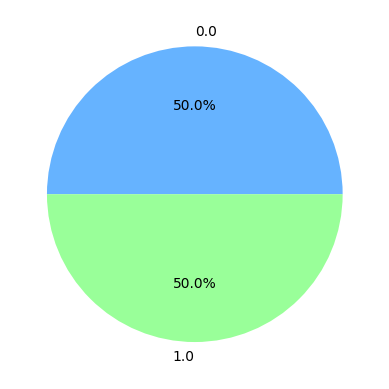
\includegraphics[width = \linewidth]{figures/binary-marker}
                \caption{pie chart shows distribution of labels in dataset of Part A}
                \label{fig:data-dist-part-a}
            \end{minipage}%
            \hfill
            \begin{minipage}{.4\linewidth}
                \centering
                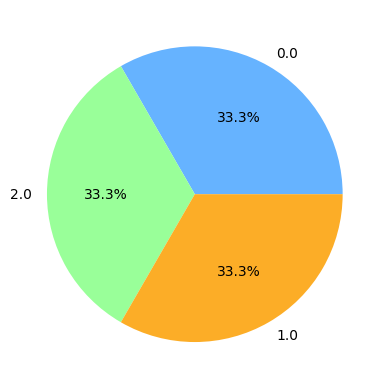
\includegraphics[width = \linewidth]{figures/multi-marker}
                \caption{pie chart shows distribution of labels in dataset of Part B}
                \label{fig:data-dist-part-b}
            \end{minipage}

        \end{figure}

    \section{ML Pipeline Design}

    It is required that the design of the ML workflow be done in Google Notebook. The links are provided in the
    \hyperref[sec:references]{References} section \cite{binary_dataset, multi_dataset}. 

        \subsection{Pre-Processing}

            Before training, data pre-processing was done to better prepare the ML models for maximum performance on
            training and better generalisation on unseen data. One of the pre-processing methods used is standardising
            the dataset so its data distribution has mean 0 and unit variance. This helps prevent a particular feature
            from overwhelming other features during training, which might contribute to unfair bias of the ML model
            towards any feature.

        \subsection{ML Models}

            For this coursework, the \verb|RandomForest| classifier from \verb|scikit-learn| was chosen and used to
            train on the dataset. Other ML models are considered, such as \verb|Logistic| regression and 
            \verb|Support Vector Machines| (\verb|SVM|) classifier, but their performance pales in comparison to 
            \verb|RandomForest| classifier, both in terms of accuracy and f1-score. This remains true for both parts
            A and B. 

        \subsection{Hyperparameter Tuning}

            The hyperparameters for \verb|RandomForest| classifier are tuned to give the best performance for it. It is
            also important to tune the hyperparameters to avoid overfitting. 
            
            The hyperparameters are not manually tuned; it is instead searched automatically via script using 
            \verb|GridSearchCV|, which is also provided from \verb|scikit-learn|. This method of hyperparameter tuning
            exhaustively searches for the best hyperparameters, by testing each combination of hyperparameters possible
            and comparing the scores of each combination. The score is user-defined, and in the case of this 
            coursework, the \verb|f1-score| is chosen over \verb|accuracy| to better reflect the generalisation 
            performance of the ML model. The best hyperparameters is then used to predict the test set.

    \section{Training Evaluation}

        Since there is no ground truth in the test set, the predicted dataset cannot be evaluated. However, the given
        training set does have ground truth, and so is used to split further into a smaller training set and a 
        validation set. The split is done with 80\% training set and 20\% validation set. This validation set is then
        used to evaluate the performance of the ML model by measuring its accuracy and f1-score. Figure 
        \ref{fig:cm-part-a} shows a confusion matrix display for part A, while figure \ref{fig:cm-part-b} shows a
        confusion matrix for part B.

        \begin{figure}[h]
            \centering

            \begin{minipage}{.4\linewidth}
                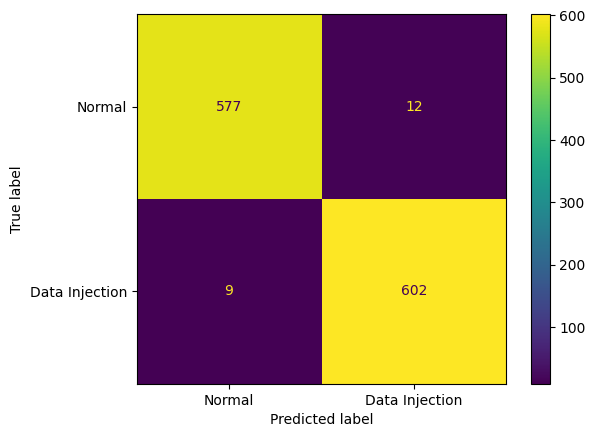
\includegraphics[width = \linewidth]{figures/binary-cm}
                \caption{confusion matrix for binary classification}
                \label{fig:cm-part-a}
            \end{minipage}%
            \hfill
            \begin{minipage}{.4\linewidth}
                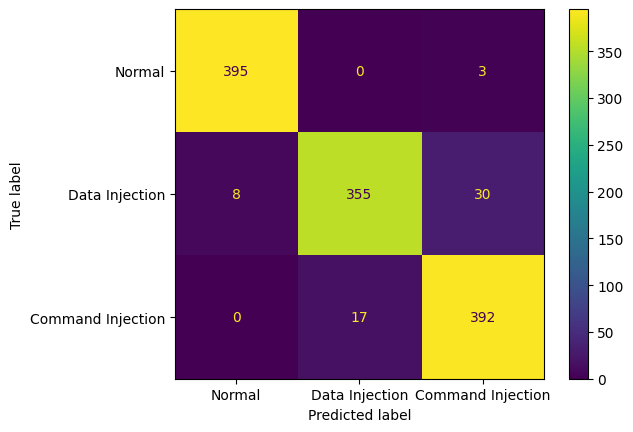
\includegraphics[width = \linewidth]{figures/multi-cm}
                \caption{confusion matrix for multi-class classification}
                \label{fig:cm-part-b}
            \end{minipage}

        \end{figure}

        From the confusion matrices, the score for both training accuracy and f1-score for part A is 98.3\%, while the
        score for training accuracy and f1-score for part B is 95.2\% and 95.1\% respectively. This shows that the
        trained \verb|RandomForest| classifier from part A performs better than the trained \verb|RandomForest| 
        classifier from part B. This can be due to the increase of labels in part B, making it more difficult for the
        ML model to generalise well on the dataset from part B.

    \section{Conclusion}

        In conclusion, the \verb|RandomForest| classifier is the best classification algorithm for this dataset. Its
        hyperparameters are further tuned to give even more performance to the classifier. Finally, the classifier is
        evaluated on validation set which is separated early on from the given dataset, since the given test set does
        not ground truth.

    \newpage

    \section{References}
    \label{sec:references}
    
        \printbibliography[heading = none]

\end{document}